\documentclass{standalone}
\usepackage{tikz}
\usetikzlibrary{positioning, fit, calc, backgrounds, shapes.geometric, arrows.meta}
\usepackage{amsmath}

\begin{document}
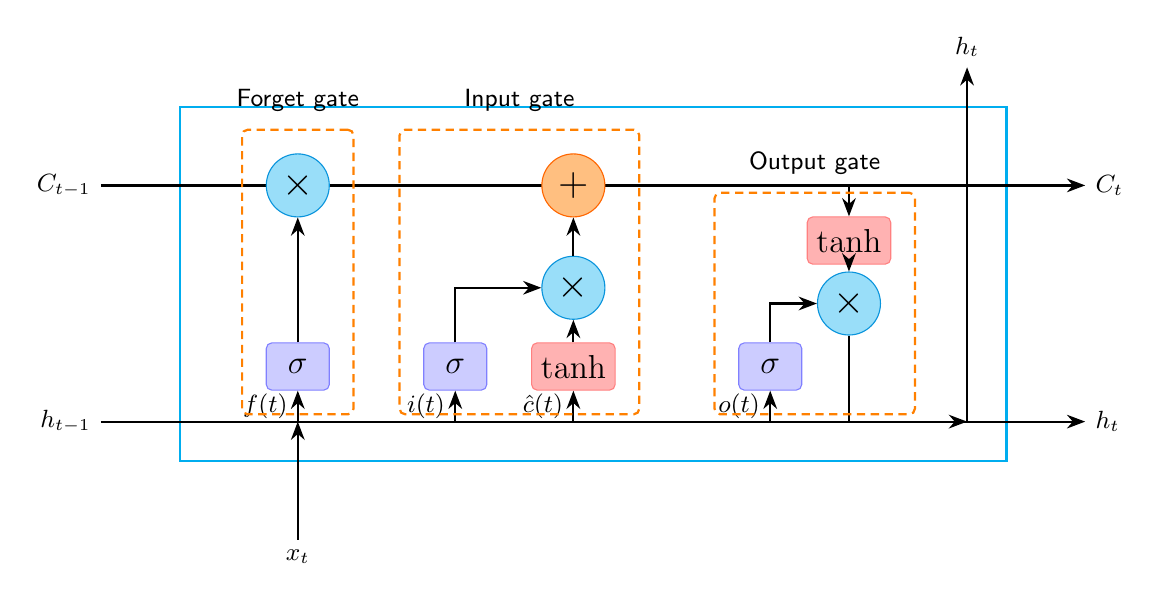
\begin{tikzpicture}[
    font=\sffamily\small,
    >=Stealth,
    op/.style={circle, draw=cyan!80!blue, fill=cyan!40, minimum size=8mm, inner sep=0pt, font=\Large\bfseries},
    add/.style={circle, draw=orange!80!red, fill=orange!50, minimum size=8mm, inner sep=0pt, font=\Large\bfseries},
    sig/.style={rectangle, draw=blue!50, fill=blue!20, rounded corners=2pt, minimum width=8mm, minimum height=6mm, font=\large},
    tanh/.style={rectangle, draw=red!50, fill=red!30, rounded corners=2pt, minimum width=8mm, minimum height=6mm, font=\large},
    gatebox/.style={rectangle, draw=orange, densely dashed, thick, inner sep=3mm, rounded corners=2pt},
    cellbox/.style={rectangle, draw=cyan, thick, inner sep=4mm, rounded corners=0pt, minimum width=10cm, minimum height=6cm}
]

% Main Cell outline (using coordinates directly)
\draw[cyan, thick] (0,0) rectangle (10.5, 4.5);

% Lines for C and h
\draw[->, thick] (-1, 3.5) node[left] {$C_{t-1}$} -- (11.5, 3.5) node[right] {$C_t$};
\draw[->, thick] (-1, 0.5) node[left] {$h_{t-1}$} -- (11.5, 0.5) node[right] {$h_t$};
\draw[->, thick] (10, 0.5) -- (10, 5) node[above] {$h_t$};

% Input x_t
\draw[->, thick] (1.5, -1) node[below] {$x_t$} -- (1.5, 0.5);

% Forget Gate
\node[sig] (f_sig) at (1.5, 1.2) {$\sigma$};
\node[op]  (f_mul) at (1.5, 3.5) {$\times$};
\draw[->, thick] (1.5, 0.5) -- (f_sig) node[midway, left] {$f(t)$};
\draw[->, thick] (f_sig) -- (f_mul);

% Input Gate
\node[sig] (i_sig) at (3.5, 1.2) {$\sigma$};
\node[op]  (i_mul) at (5.0, 2.2) {$\times$};
\node[tanh] (i_tanh) at (5.0, 1.2) {$\tanh$};
\node[add] (i_add) at (5.0, 3.5) {$+$};

\draw[->, thick] (3.5, 0.5) -- (i_sig) node[midway, left] {$i(t)$};
\draw[->, thick] (i_sig) |- (i_mul);
\draw[->, thick] (5.0, 0.5) -- (i_tanh) node[midway, left] {$\hat{c}(t)$};
\draw[->, thick] (i_tanh) -- (i_mul);
\draw[->, thick] (i_mul) -- (i_add);

% Output Gate
\node[sig] (o_sig) at (7.5, 1.2) {$\sigma$};
\node[tanh] (o_tanh) at (8.5, 2.8) {$\tanh$};
\node[op]  (o_mul) at (8.5, 2.0) {$\times$};

\draw[->, thick] (7.5, 0.5) -- (o_sig) node[midway, left] {$o(t)$};
\draw[->, thick] (o_sig) |- (o_mul);
\draw[->, thick] (8.5, 3.5) -- (o_tanh);
\draw[->, thick] (o_tanh) -- (o_mul);
\draw[->, thick] (o_mul) |- (10, 0.5);

% Grouping Boxes
\node[gatebox, fit=(f_sig) (f_mul)] (forget_box) {};
\node[above=1mm of forget_box] {Forget gate};

\node[gatebox, fit=(i_sig) (i_tanh) (i_add)] (input_box) {};
\node[above=1mm of input_box] {Input gate};

\node[gatebox, fit=(o_sig) (o_tanh) (o_mul)] (output_box) {};
\node[above=1mm of output_box] {Output gate};

\end{tikzpicture}
\end{document}
